% This flow chart is created by the author

% adjustbox is used to limit the figure inside the page
% -- means normal arrow
%  -| horizontal followed by the vertical arrow
%  |- vertical followed by the horizontal arrow


\begin{figure}

    \begin{center}
        \begin{adjustbox}{max height=\textheight, center, width=0.8\textwidth}
            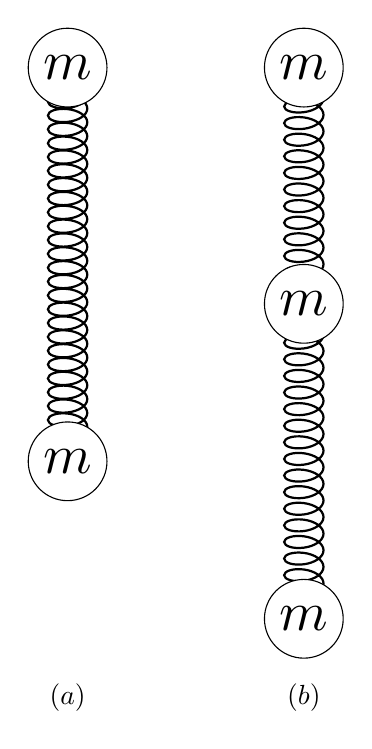
\begin{tikzpicture}
\tikzstyle{spring}=[thick,decorate,decoration={aspect=.5, segment length=5, amplitude=2.5mm,coil, post length=0, pre length=0}]
   % \draw[pattern={north east lines}] (-1,5.2) rectangle (1,5.4);
    \draw [spring] (0,0) -- (0,-5);
    \node[] at (0,-8) {$(a)$};
    \draw [fill=white] (0,0) circle (.5) node[draw=none,inner sep = 0,scale=2,text=black]{$m$};
    \draw [fill=white] (0,-5) circle (.5) node[draw=none,inner sep = 0,scale=2,text=black]{$m$};
%________________________________________________________________%
\tikzstyle{spring}=[thick,decorate,decoration={aspect=.5, segment length=6, amplitude=2.5mm,coil, post length=0, pre length=0}]
    \draw [spring] (3,0) -- (3,-3);
   \draw [fill=white] (3,0) circle (.5) node[draw=none,inner sep = 0,scale=2,text=black]{$m$};
    \tikzstyle{spring}=[thick,decorate,decoration={aspect=.5, segment length=6, amplitude=2.5mm,coil, post length=0, pre length=0}]
    \draw [spring] (3,-3) -- (3,-7);
    \draw [fill=white] (3,-3) circle (.5) node[draw=none,inner sep = 0,scale=2,text=black]{$m$};
    \draw [fill=white] (3,-7) circle (.5) node[draw=none,inner sep = 0,scale=2,text=black]{$m$};
    \node[] at (3,-8) {$(b)$};
            \end{tikzpicture}
        \end{adjustbox}
    \end{center}
    \caption{Caption for flowchart.}
    \label{fig:figure1}
\end{figure}